\chapter{Medición de Inductancias}
    \section{Introducción}
    \label{sec:ej3Intro}
    \begin{figure}[h]
        \begin{center}
            \begin{circuitikz}[scale = 0.75, transform shape]
    \draw
    (0,0)
    to [sV, l=$V_g$] (0,8)
    to (4,8)
    to [R, l=$R_1$] (4,4)
    to [C, l=$C_3$] (4,2)
    to [R, l=$R_3$] (4,0) to (0,0)
    (4,8) to (8,8)
    to [L, l=$L_x$] (8,4)
    to [R, l=$R_4$] (8,0) to (4,0)
    (4,4) to [voltmeter, l=$V_d$] (8,4)
    (8,7) to (7,7) to [R, l=$R_x$] (7,5) to (8,5)
    ;
\end{circuitikz}
\caption{Puente de Hay}
\label{fig:Hay}
        \end{center}
        
    \end{figure}
    En principio, dado que la bobina entregada tiene un factor de calidad
    $Q_N\approx53$ a una frecuencia $f=10\si{\kilo\hertz}$, se decidió utilizar un
    puente de Hay, como visto en la Figura \ref{fig:Hay}, en lugar de un puente de
    Maxwell, el cual funciona apropiadamente en un rango de $Q\in(1,10)$.
    
    \section{Especificaciones}
    \label{sec:ej3Specs}
    Se desea que el rango de inductancias medibles sea $L_x\in[0.4\si{\milli\henry};
    2.1\si{\milli\henry}]$. Además, el rango de Q también debe ser $Q\in[0.25Q_N; Q_N]$.
    Estas características se deben cumplir cuando $f=10\si{\kilo\hertz}$ y $Q_N$ es
    el factor de calidad de la bobina patrón.
    
    \section{Diseño}
    \label{sec:ej3Design}
    Para la realización del puente, se tuvieron en cuenta las ecuaciones (\ref{eq:ej3V}),
    (\ref{eq:ej3L}), (\ref{eq:ej3Q}) y (\ref{eq:ej3R}).
    \begin{equation}
        V_d=\frac{(R_3 + \frac{1}{C_3})}{(R_1+R_3 + \frac{1}{C_3})} - \frac{R_4}{((\frac{1}{R_x}+\frac{1}{sL_x})^{-1}+R_4)} \times V_g
        \label{eq:ej3V}
    \end{equation}
    \begin{equation}
        L_x = C_3 R_1 R_4
        \label{eq:ej3L}
    \end{equation}
    \begin{equation}
        Q_x=\frac{1}{2 \pi f C_3 R_3}
        \label{eq:ej3Q}
    \end{equation}
    \begin{equation}
        R_x=\frac{R_1 R_4}{R_3}
        \label{eq:ej3R}
    \end{equation}

    Observando las ecuaciones (\ref{eq:ej3L}) y (\ref{eq:ej3Q}), se define que las variables
    de ajuste serán $R_1$ y $R_3$, dado que intentar variar $C_3$ sería demasiado 
    complicado y afecta a ambos $L_x$ y $Q_x$. Además, aunque $R_4$ también parece
    ser un candidato viable, es preferible mantenerlo constante para que la relación
    (\ref{eq:ej3A}) se mantenga constante.
    
    \begin{equation}
        A=\frac{Z_4}{Z_2}=\frac{Z_3}{Z_1}
        \label{eq:ej3A}
    \end{equation}
    
    Teniendo en cuenta las variables a ser modificadas, los márgenes de operación
    descriptos en la sección \ref{sec:ej3Specs} calcularon los valores para cada componente.
    De las expresiones anteriores se obtiene que

    \begin{equation}
        R_1 \in [\frac{L_{min}}{C_3 R_4};\frac{L_{MAX}}{C_3 R_4}] = [1.8182\si{\kilo\ohm}; 9.5455\si{\kilo\ohm}]
        \label{eq:ej3ranR1}
    \end{equation}

    \begin{equation}
        R_3 \in [\frac{1}{2 \pi f Q_{MAX}}; \frac{1}{2 \pi f Q_{min}}] = [136.50\si{\ohm}; 545.98\si{\ohm}]
        \label{eq:ej3ranR3}
    \end{equation}

    Dados los rangos obtenidos en las expresiones \ref{eq:ej3ranR1} y \ref{eq:ej3ranR3}, y considerando
    los componentes disponibles, se eligieron los valores en el cuadro \ref{tab:ej3Specs} para construir
    el puente y se obtiene el diseño en la Figura \ref{fig:ej3Design}.

    \begin{table}[h]
        \begin{center}
            \begin{tabular}{|c|c|}
                \hline
                Componente & Valor \\
                \hline
                $R_1$ & $[1.8\si{\kilo\ohm} \rightarrow 11.8\si{\kilo\ohm}]$\\
                $R_3$ & $[100\si{\ohm} \rightarrow 600\si{\ohm}]$\\
                $R_4$ & $100\si{\ohm}$\\
                $C_3$ & $2.2\si{\nano\farad}$\\
                \hline
            \end{tabular}
            \caption{Especificaciones elegidas para los componentes}
            \label{tab:ej3Specs}
        \end{center}
    \end{table}

    \begin{figure}[ht!]
        \begin{center}
            \begin{circuitikz}[scale = 0.75, transform shape]
    \draw
    (0,0) to [sV, l=$V_g$] (0,12)
    (4,0)
    to [R , l=$200\si{\ohm}$] (4,2)
    to [vR, l=$1\si{\kilo\ohm}$] (4,4)
    to [C , l=$1.2\si{\nano\farad}$] (4,6)
    to [R , l=$200\si{\ohm}$] (4,8)
    to [vR, l=$100\si{\ohm}$] (4,10)
    to [vR, l=$1\si{\kilo\ohm}$] (4,12)
    (8,0)
    to [R , l=$1\si{\kilo\ohm}$] (8,3)
    to [R , l=$560\si{\ohm}$] (8,6)
    to [L , l=$L_x$] (8,12)
    (8,8) to (7,8) to [R, l=$R_x$] (7,10) to (8,10)
    (0,12) to (8,12)
    (0,0) to (8,0)
    (4,6) to [voltmeter, l=$V_d$] (8,6)
    ;
\end{circuitikz}
\caption{Puente diseñado}
\label{fig:ej3Design}
        \end{center}
    \end{figure}

    Los resistores variables de menor tamaño fueron puestos con el propósito de reducir
    la sensibilidad del puente respecto a $R_1$. Además, se prefirió elegir las resistencias de tal forma que
    abarquen un rango levemente mayor al calculado. Se utilizó un preset de $20\si{\kilo\ohm}$ dada la falta
    de uno de $10\si{\kilo\ohm}$.

    \section{Simulación y Sensibilidades}

    En las figuras \ref{fig:ej3Vd:patron} y \ref{fig:ej3Vd:min-MAX} se puede observar el comportamiento
    de $V_d$ en función de las resistencias $R_1$ y $R_3$ para distintas inductancias de prueba.
    Es notable que las resistencias afectan de manera dispareja a $V_d$.
    
    \begin{figure}[ht]
        \begin{center}
            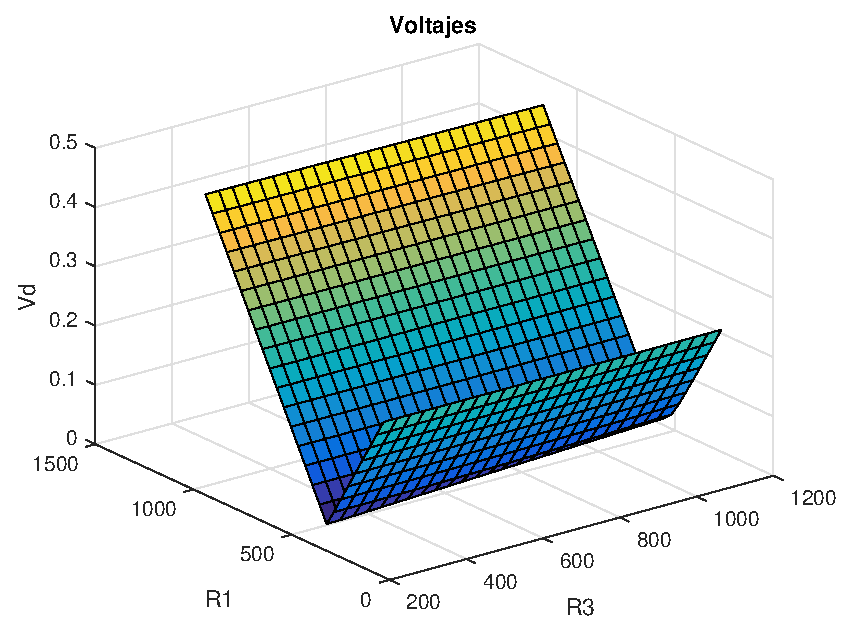
\includegraphics[width=0.45\linewidth]{MATLAB/ej3Vd}
            \caption{$L_x=0.9713\si{\milli\henry}$; $Q_x=53$(Componente Patrón)}
            \label{fig:ej3Vd:patron}
        \end{center}
    \end{figure}

    \begin{figure}[ht]
        \begin{center}
            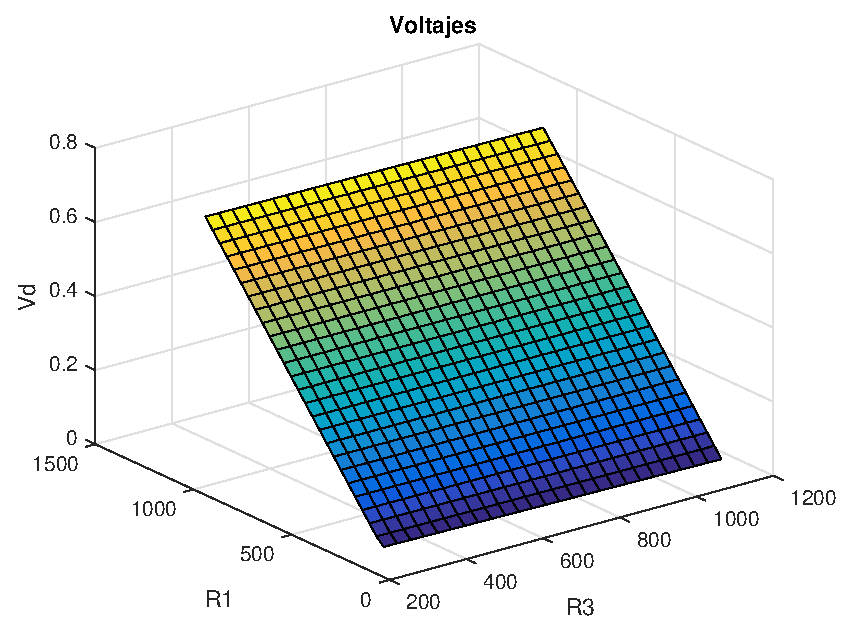
\includegraphics[width=0.4\linewidth]{MATLAB/ej3Vdmin}
            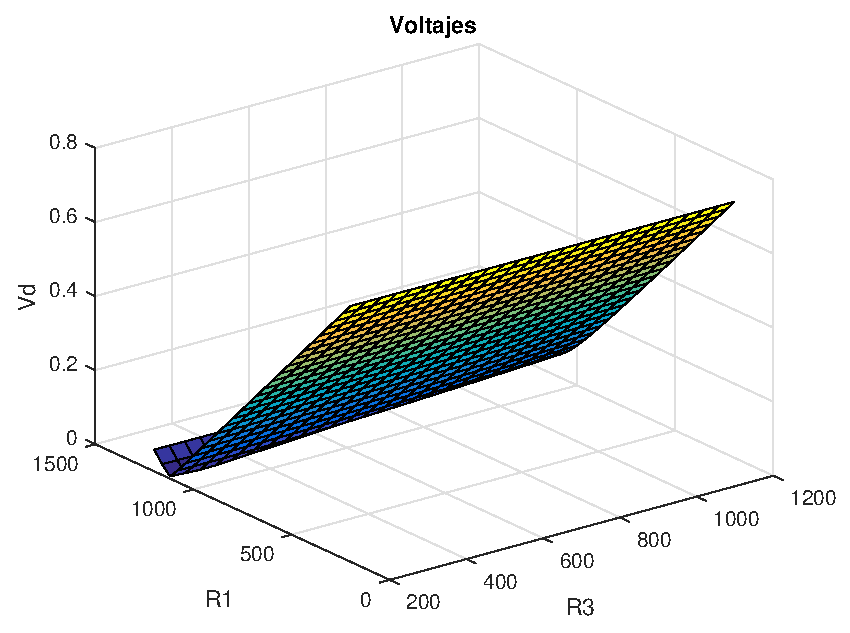
\includegraphics[width=0.4\linewidth]{MATLAB/ej3Vdmax}
            \caption{$L_x=0.4\si{\milli\henry}$; $Q_x=53$/$L_x=2.1\si{\milli\henry}$; $Q_x=13.25$}
            \label{fig:ej3Vd:min-MAX}
        \end{center}
    \end{figure}

    Además, como se ve en las figuras \ref{fig:ej3dVd:patron}, \ref{fig:ej3dVd:min} y \ref{fig:ej3dVd:max}, 
    aunque los valores de las sensibilidades para los diferentes casos son diferentes, en todo
    momento se encuentran dentro de aproximadamente el mismo orden de magnitud, debido a los resistores
    variables de baja amplitud colocados en el diseño. Considerando esto, se puede concluir que $R_3$
    puede ser usada como una resistencia de ajuste fino, mientras que $R_1$ sería una de ajuste grueso.

    Si es necesario, incluso se pueden hacer ajuster finos con la resistencia variable de $100\si{\ohm}$
    colocada en $R_1$.

    Los gráficos de las sensibilidades fueron creados a partir de sus fórmulas analíticas (ecuaciones \ref{eq:ej3dVdR3} y \ref{eq:ej3dVdR1}).

    \begin{equation}
        |\Delta V_d| = \left| \frac{1}{(1+\frac{Z_1}{Z_3})(\frac{Z_4}{Z_2} + 1)} \cdot \frac{\Delta R_3}{Z_3} \right| \cdot V_g 
        \label{eq:ej3dVdR3}
    \end{equation}

    \begin{equation}
        |\Delta V_d| = \left| \frac{1}{(\frac{Z_3}{Z_1}+1)(1+\frac{Z_2}{Z_4})} \cdot \frac{\Delta R_1}{Z_1} \right| \cdot V_g
        \label{eq:ej3dVdR1}
    \end{equation}

    \begin{figure}[ht!]
        \begin{center}
            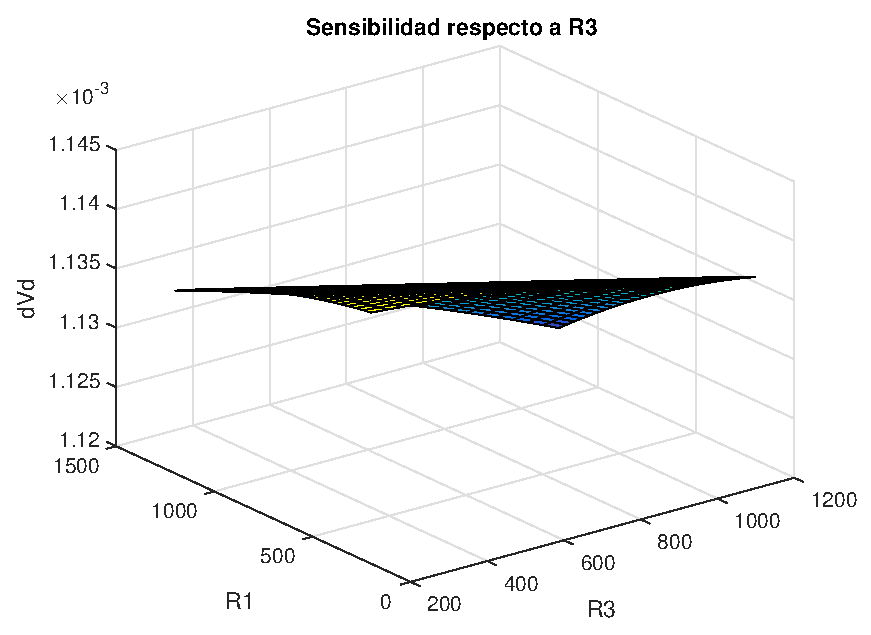
\includegraphics[width=0.4\linewidth]{MATLAB/ej3dVd3}
            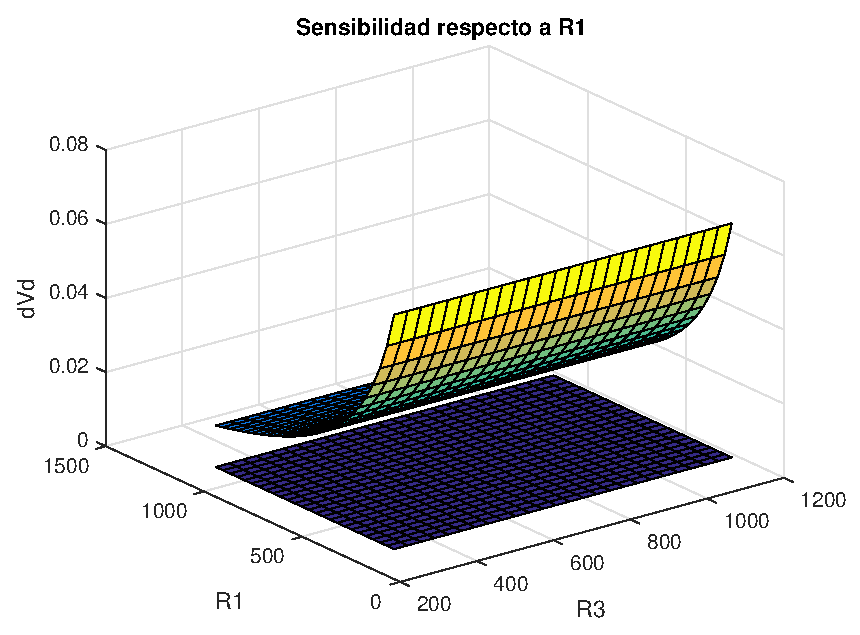
\includegraphics[width=0.4\linewidth]{MATLAB/ej3dVd1}
            \caption{$L_x=0.9713\si{\milli\henry}$; $Q_x=53$(Componente Patrón)}
            \label{fig:ej3dVd:patron}
        \end{center}
    \end{figure}

    \begin{figure}[ht!]
        \begin{center}
            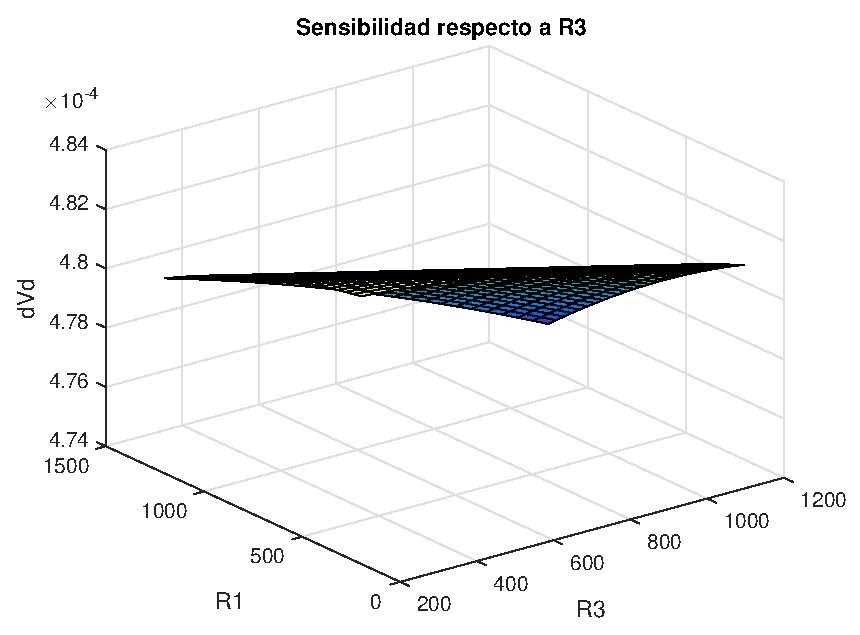
\includegraphics[width=0.4\linewidth]{MATLAB/ej3dVd3min}
            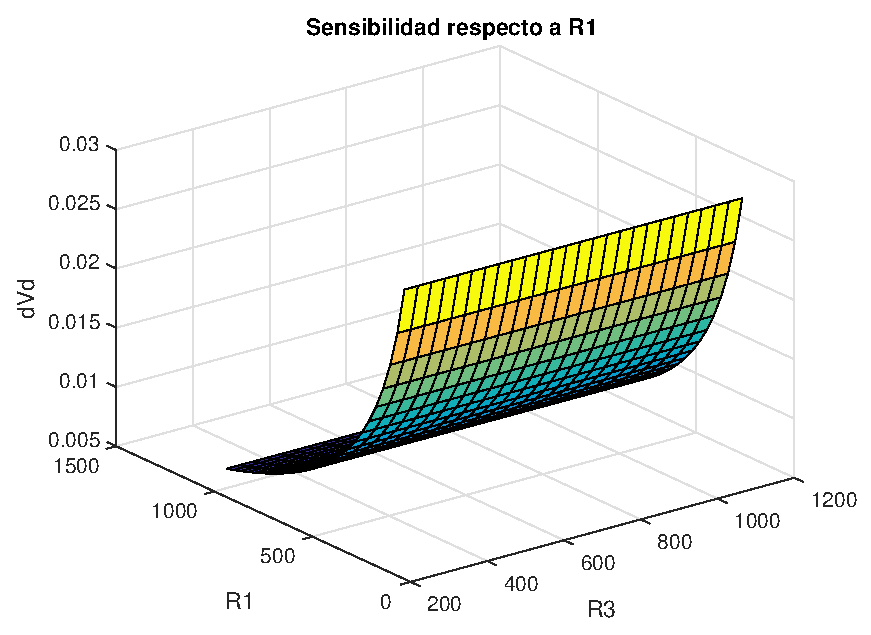
\includegraphics[width=0.4\linewidth]{MATLAB/ej3dVd1min}
            \caption{$L_x=0.4\si{\milli\henry}$; $Q_x=53$}
            \label{fig:ej3dVd:min}
        \end{center}
    \end{figure}

    \begin{figure}[ht!]
        \begin{center}
            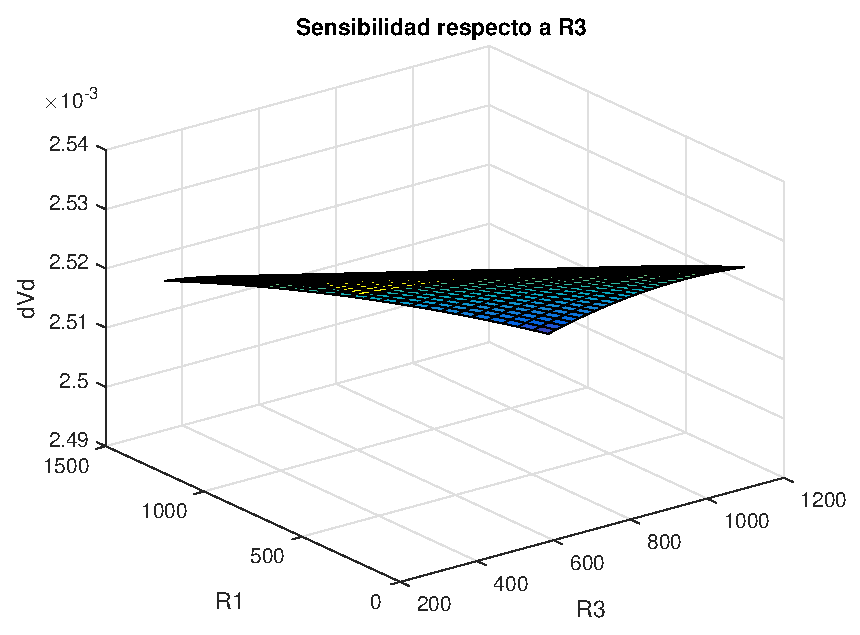
\includegraphics[width=0.4\linewidth]{MATLAB/ej3dVd3max}
            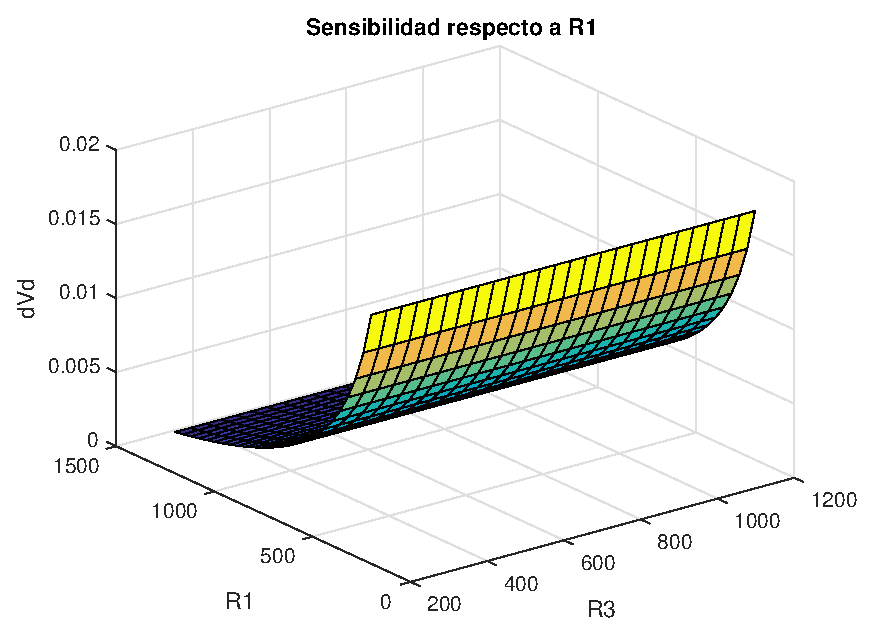
\includegraphics[width=0.4\linewidth]{MATLAB/ej3dVd1max}
            \caption{$L_x=2.1\si{\milli\henry}$; $Q_x=13.25$}
            \label{fig:ej3dVd:max}
        \end{center}
    \end{figure}

    \newpage
    \section{Manual de Uso}
    El puente diseñado permite medir inductancias tales que $L_x\in[0.4\si{\milli\henry};
    2.1\si{\milli\henry}]$ y $Q\in[0.25Q_N; Q_N]$ para $f=10\si{\kilo\hertz}$. 
    Instrucciones:
    \begin{enumerate}
        \item Llevar al mínimo todos los presets de $R_1$ y $R_3$.
        \item Minimizar $V_d$ utilizando el preset de $20\si{\kilo\ohm}$ de $R_1$.
        \item Minimizar $V_d$ utilizando el preset de $1\si{\kilo\ohm}$ de $R_1$.
        \item Minimizar $V_d$ utilizando el preset de $100\si{\ohm}$ de $R_1$.
        \item Minimizar $V_d$ utilizando el preset de $R_3$.
        \item Minimizar $V_d$ alternando entre los ajustes finos de $R_1$ y $R_3$.
        \item Medir las resistencias finales y calcular $L_x$, $Q_x$ y $R_x$.
    \end{enumerate}

    Alternativamente a medir las resistencias finales, el uso de los presets puede hacerse
    contando el número de vueltas dadas al ajuste para tomar los valores de las resistencias
    finales. Se recomienda el uso de vueltas enteras, ya que con esas diferencias de paso
    fueron calculadas las sensibilidades.

    Por otro lado, dado el uso del preset de $20\si{\kilo\ohm}$ en lugar del de $10\si{\kilo\ohm}$,
    se advierte no pasar de las 13 vueltas, ya que se encuentra fuera del rango de resistencias
    del puente.

    \begin{table}[h]
        \begin{center}
            \begin{tabular}{|l|r|}
                \hline
                Especificación & Valor \\
                \hline
                Rango de $L_x$ & $[0.4;2.1]\si{\milli\henry}$ \\
                Rango de $Q_x$ & $ [13.25; 53] $ \\
                Frecuencia & $10\si{\kilo\hertz}$\\
                $V_g$ & $10\si{\volt}$\\
                $C_3$ & $2.2\si{\nano\farad}$\\
                \hline
            \end{tabular}
            \begin{tabular}{|l|r|}
                \hline
                Especificación & Valor \\
                \hline
                $R_1$ & $[1.8;11.8]\si{\kilo\ohm}$\\
                $R_3$ & $[100;600]\si{\ohm}$\\
                $\Delta R_1$ & $4\si{\ohm}$ \\
                $\Delta R_3$ & $20\si{\ohm}$ \\
                $R_4$ & $100\si{\ohm}$\\
                \hline
            \end{tabular}
            \caption{Especificaciones del Puente}
            \label{tab:ej3specFin}
        \end{center}
    \end{table}

    \section{Mediciones}
    Armado el puente en placa experimental, se completó la tabla \ref{tab:ej3d}:
    \pgfplotstableset{
    alias/nom/.initial = Nominal,
    alias/obs/.initial = Observaciones,
}
\pgfplotstabletypeset[
    %General%
    col sep = comma,
    string type,
    columns = {nom,L1,Q1,P1,L10,Q10,P10,L100,Q100,P100,obs},
    every head row/.style={
        before row = {
            \toprule
            Valor & \multicolumn{3}{c|}{$f = 1\si{k\hertz}$} & \multicolumn{3}{c|}{$f = 10\si{k\hertz}$} & \multicolumn{3}{c|}{$f = 100\si{k\hertz}$} &\\
        },
        after row = {\midrule}
    },
    column type/.add = {|}{},
    every last column/.style={
        column type/.add={}{|},
    },
    every last row/.style={after row=\bottomrule},
    %Especifico cada columna%
    columns/nom/.style={
        column name = Nominal,
    },
    columns/obs/.style={
        column name = Observaciones,
    },
    columns/L1/.style={
        column name = $L$,
    },
    columns/Q1/.style={
        column name = $Q$,
    },
    columns/P1/.style={
        column name = $P$,
    },
    columns/L10/.style={
        column name = $L$,
    },
    columns/Q10/.style={
        column name = $Q$,
    },
    columns/P10/.style={
        column name = $P$,
    },
    columns/L100/.style={
        column name = $L$,
    },
    columns/Q100/.style={
        column name = $Q$,
    },
    columns/P100/.style={
        column name = $P$,
    },
    ]{tabla3d.csv}
\caption{Resultados de las mediciones}
\label{tab:ej3}

    Se repitieron las mediciones con el analizador de impedancias y se llenó la tabla \ref{tab:ej3e}
    \pgfplotstableset{
    alias/nom/.initial = Nominal,
}
\begin{table}[ht]
    \begin{center}
        \pgfplotstabletypeset[
            %General%
            col sep = comma,
            string type,
            columns = {nom,L1,Q1,L10,Q10,L100,Q100},
            every head row/.style={
                before row = {
                    \toprule
                    Valor & \multicolumn{2}{c|}{$f = 1\si{k\hertz}$} & \multicolumn{2}{c|}{$f = 10\si{k\hertz}$} & \multicolumn{2}{c|}{$f = 100\si{k\hertz}$}\\
                },
                after row = {\midrule}
            },
            column type/.add = {|}{},
            every last column/.style={
                column type/.add={}{|},
            },
            every last row/.style={after row=\bottomrule},
            %Especifico cada columna%
            columns/nom/.style={
                column name = Nominal,
            },
            columns/L1/.style={
                column name = $L(\si{\milli\henry})$,
            },
            columns/Q1/.style={
                column name = $Q$,
            },
            columns/L10/.style={
                column name = $L(\si{\milli\henry})$,
            },
            columns/Q10/.style={
                column name = $Q$,
            },
            columns/L100/.style={
                column name = $L(\si{\milli\henry})$,
            },
            columns/Q100/.style={
                column name = $Q$,
            },
            ]{tabla3e.csv}
        \caption{Mediciones con el analizador de impedancias}
        \label{tab:ej3e}
    \end{center}
\end{table}


    \section{Errores}
    Se calculó analíticamente el error en las ecuaciones \ref{eq:ej3errL} y \ref{eq:ej3errQ}.
    \begin{equation*}
        \begin{split}
            \Delta L_x &=\left| \frac{\delta L_x}{\delta R_1} \right| \cdot \Delta R_1\\
                       &= C_3 R_4 \cdot \Delta R_1
        \end{split}
    \end{equation*}

    \begin{equation}
        \Rightarrow\frac{\Delta L_x}{L_x} = \frac{\Delta R_1}{R_1}
        \label{eq:ej3errL}
    \end{equation}

    \begin{equation*}
        \begin{split}
            \Delta Q_x &= \left| \frac{\delta Q_x}{\delta R_3} \right| \cdot \Delta R_3\\
                       &= \frac{1}{ 2 \pi f C_3 {R_3}^2} \cdot \Delta R_3
        \end{split}
    \end{equation*}

    \begin{equation}
        \Rightarrow\frac{\Delta Q_x}{Q_x} = \frac{\Delta R_3}{R_3}
        \label{eq:ej3errQ}
    \end{equation}

    (LLenar con tabla de errores)
    % \pgfplotstableset{
    alias/nom/.initial = Nominal,
}
\begin{table}[ht]
    \begin{center}
        \pgfplotstabletypeset[
            %General%
            col sep = comma,
            string type,
            columns = {nom,L1,Q1,L10,Q10,L100,Q100},
            every head row/.style={
                before row = {
                    \toprule
                    Valor & \multicolumn{2}{c|}{$f = 1\si{k\hertz}$} & \multicolumn{2}{c|}{$f = 10\si{k\hertz}$} & \multicolumn{2}{c|}{$f = 100\si{k\hertz}$}\\
                },
                after row = {\midrule}
            },
            column type/.add = {|}{},
            every last column/.style={
                column type/.add={}{|},
            },
            every last row/.style={after row=\bottomrule},
            %Especifico cada columna%
            columns/nom/.style={
                column name = Nominal,
            },
            columns/L1/.style={
                column name = $L$,
            },
            columns/Q1/.style={
                column name = $Q$,
            },
            columns/L10/.style={
                column name = $L$,
            },
            columns/Q10/.style={
                column name = $Q$,
            },
            columns/L100/.style={
                column name = $L$,
            },
            columns/Q100/.style={
                column name = $Q$,
            },
            ]{tablaErr.csv}
        \caption{Errores experimentales para las mediciones}
        \label{tab:ej3err}
    \end{center}
\end{table}


    \section{Conclusiones}